
\documentclass[fleqn,addpoints]{exam}

\usepackage{graphicx}
\usepackage{float}
\usepackage{amsmath}
\usepackage{cancel}
\usepackage{polynom}
\usepackage{caption}

\printanswers

\ifprintanswers 
\usepackage{2in1, lscape} 
\fi

\title{Math 115 Homework 14}
\date{January 15, 2011}

\begin{document}

\maketitle

\section{Administrative}

There will be no class on 1/18 and 1/25.  The Chapter 2 exam will be on 2/1. 

\section{Homework}
Faires/DeFranza, p. 154, 7-10, 13

\ifprintanswers
\else
\section{Review}
The exam will cover Larsen/Hostetler Sections 2.2-2.6.  Or, if you prefer, Faires/DeFranza, Chapter 2.

To practice for the exam, you should take a look at the Chapter 2 review exercises, pp. 280-283.  You should know how to
do: 33-38, 43-60, 88-126, 142-144, 146-147.  You don't have to do all of these, of course, but you should take a look at
a few problems from each category to review.
\fi

\section{Page 154}

I seem to have a problem typing the page number correctly lately.  This week was supposed to be page 154, not 134.

\begin{description}
\item[7]
\begin{figure}[H]
  \centering
  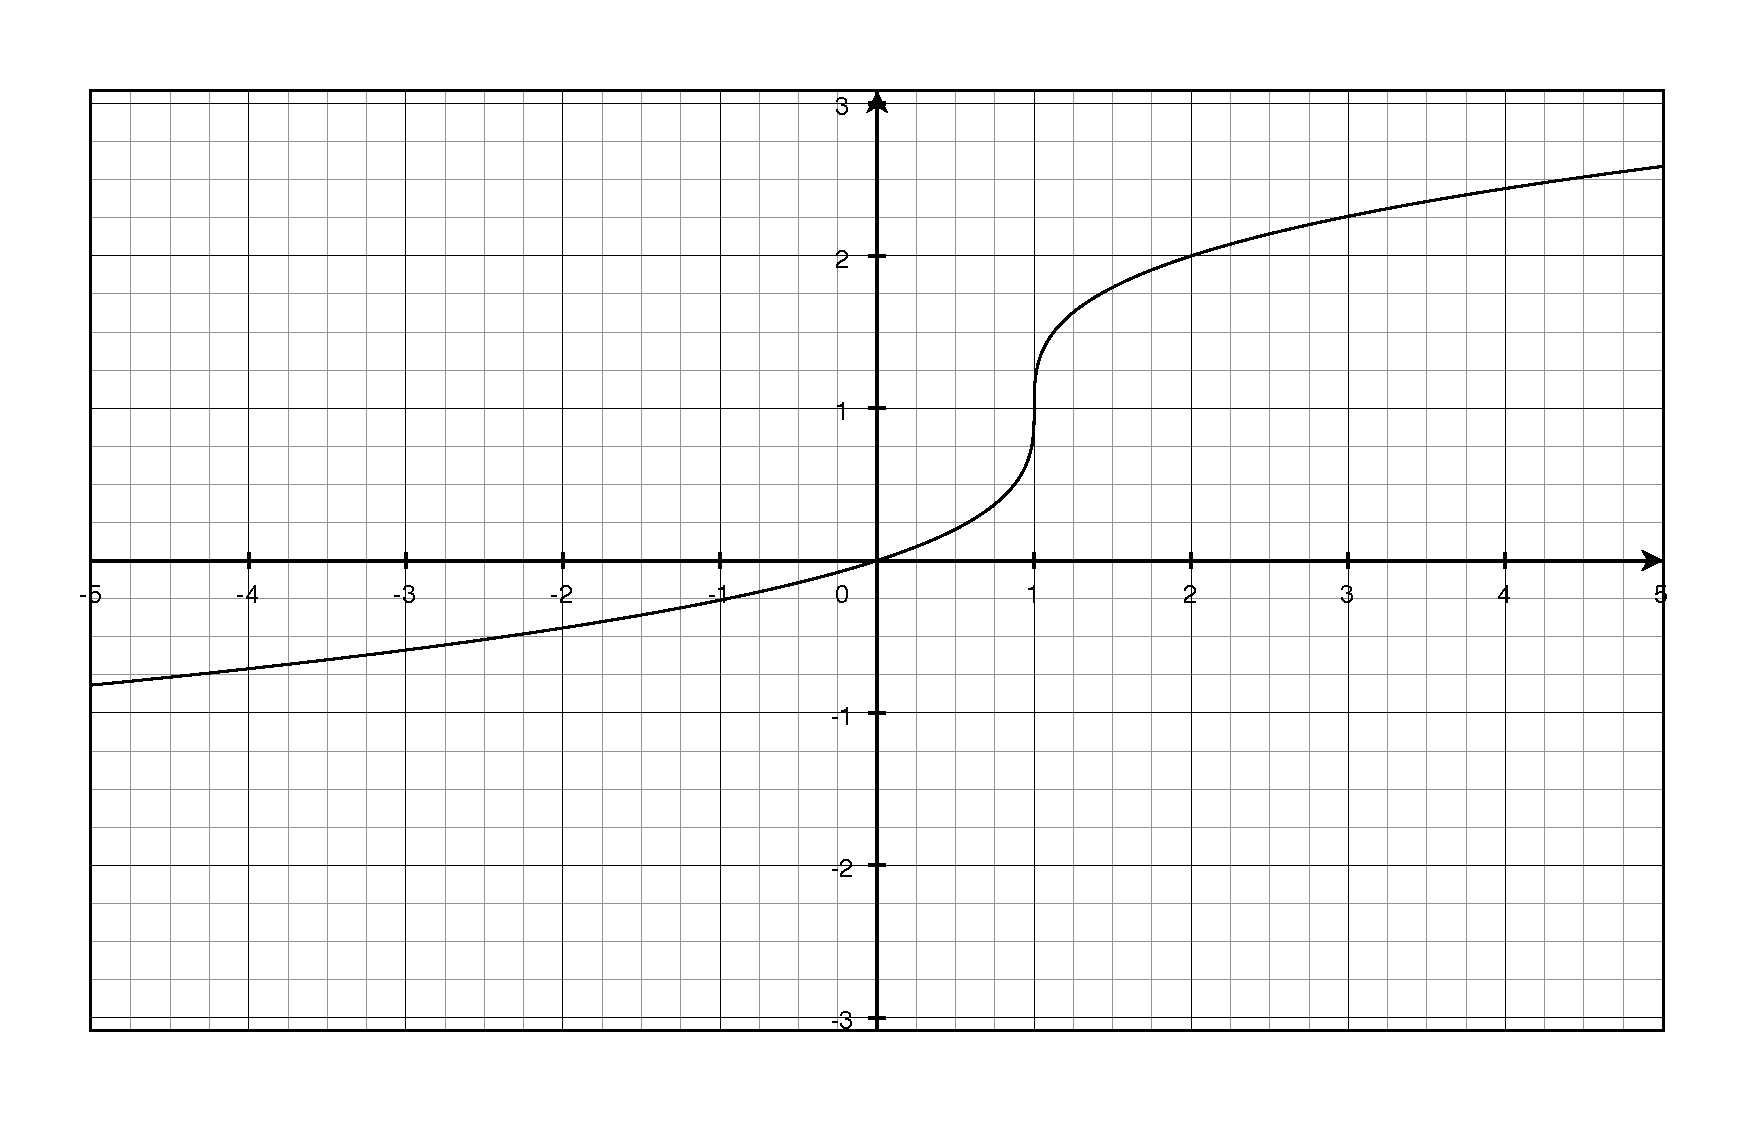
\includegraphics[scale=.3]{question7.eps}
  \caption*{Question 7}
\end{figure}

\item[8]
\begin{figure}[H]
  \centering
  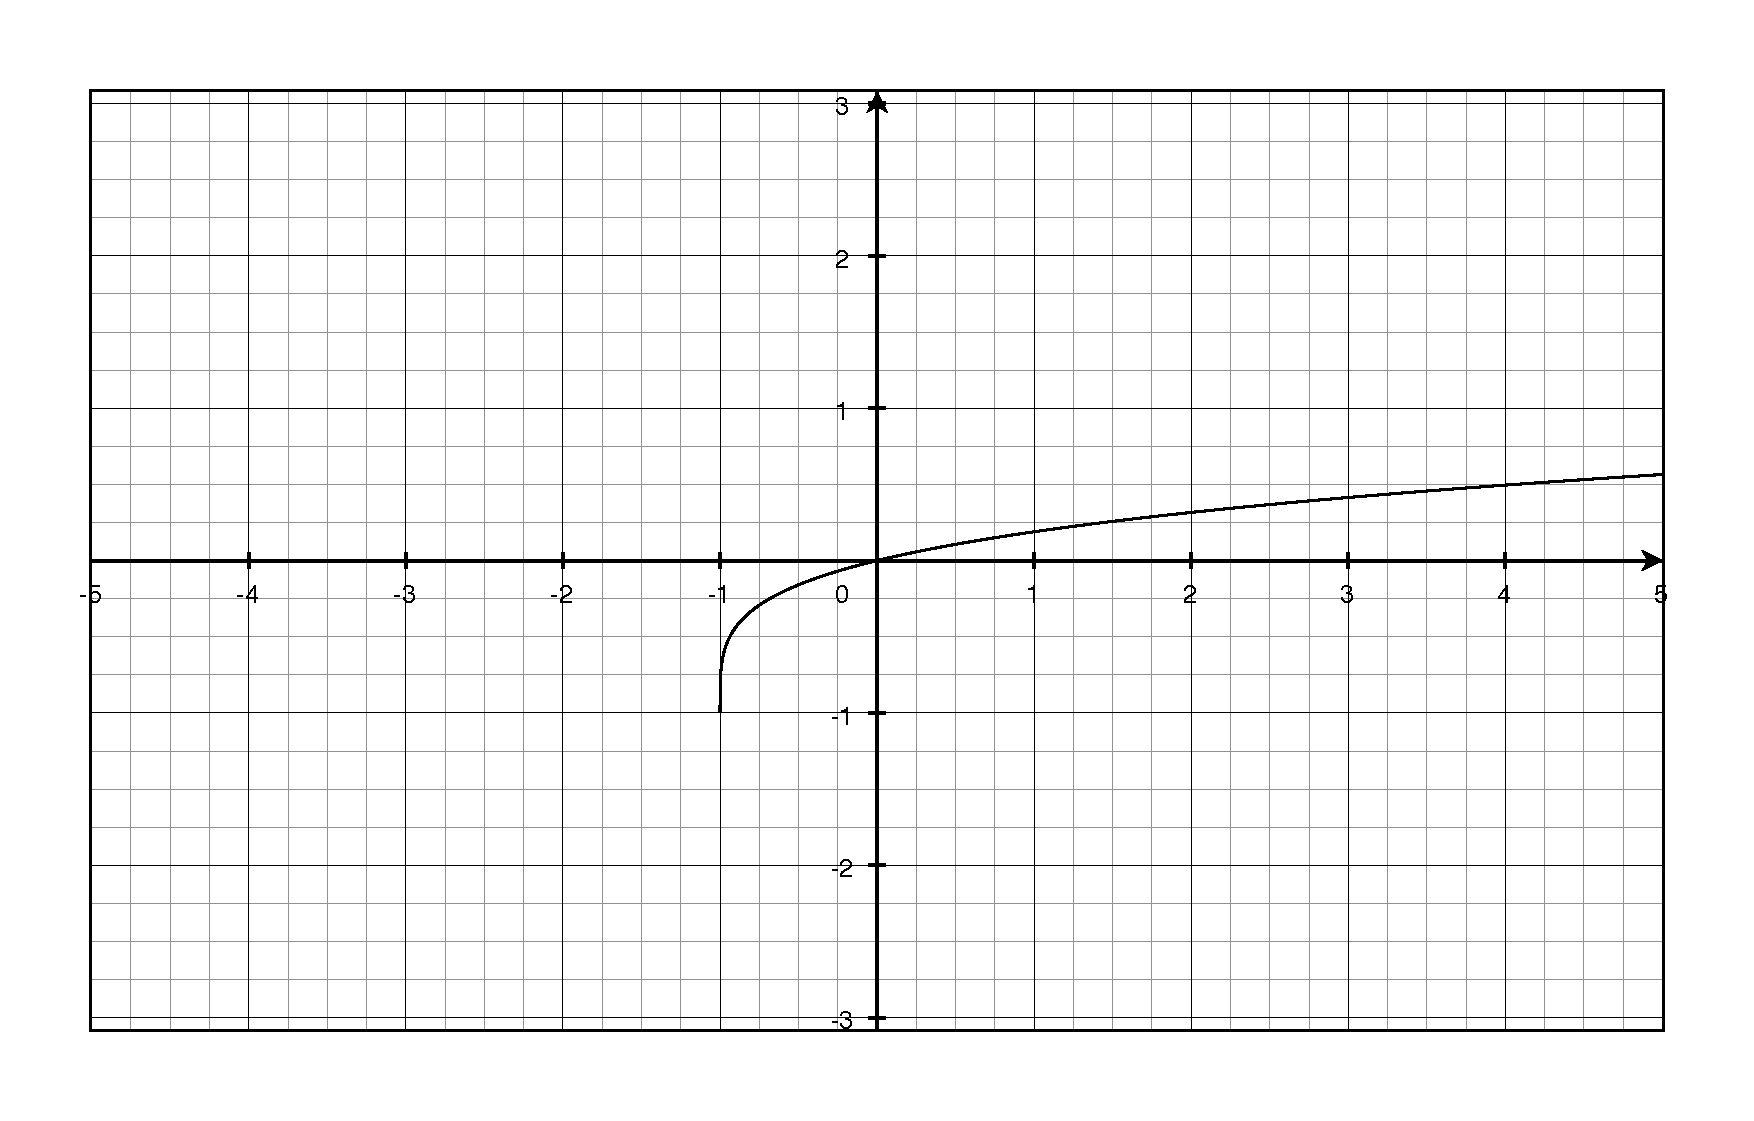
\includegraphics[scale=.3]{question8.eps}
  \caption*{Question 8}
\end{figure}

\item[9]
\begin{figure}[H]
  \centering
  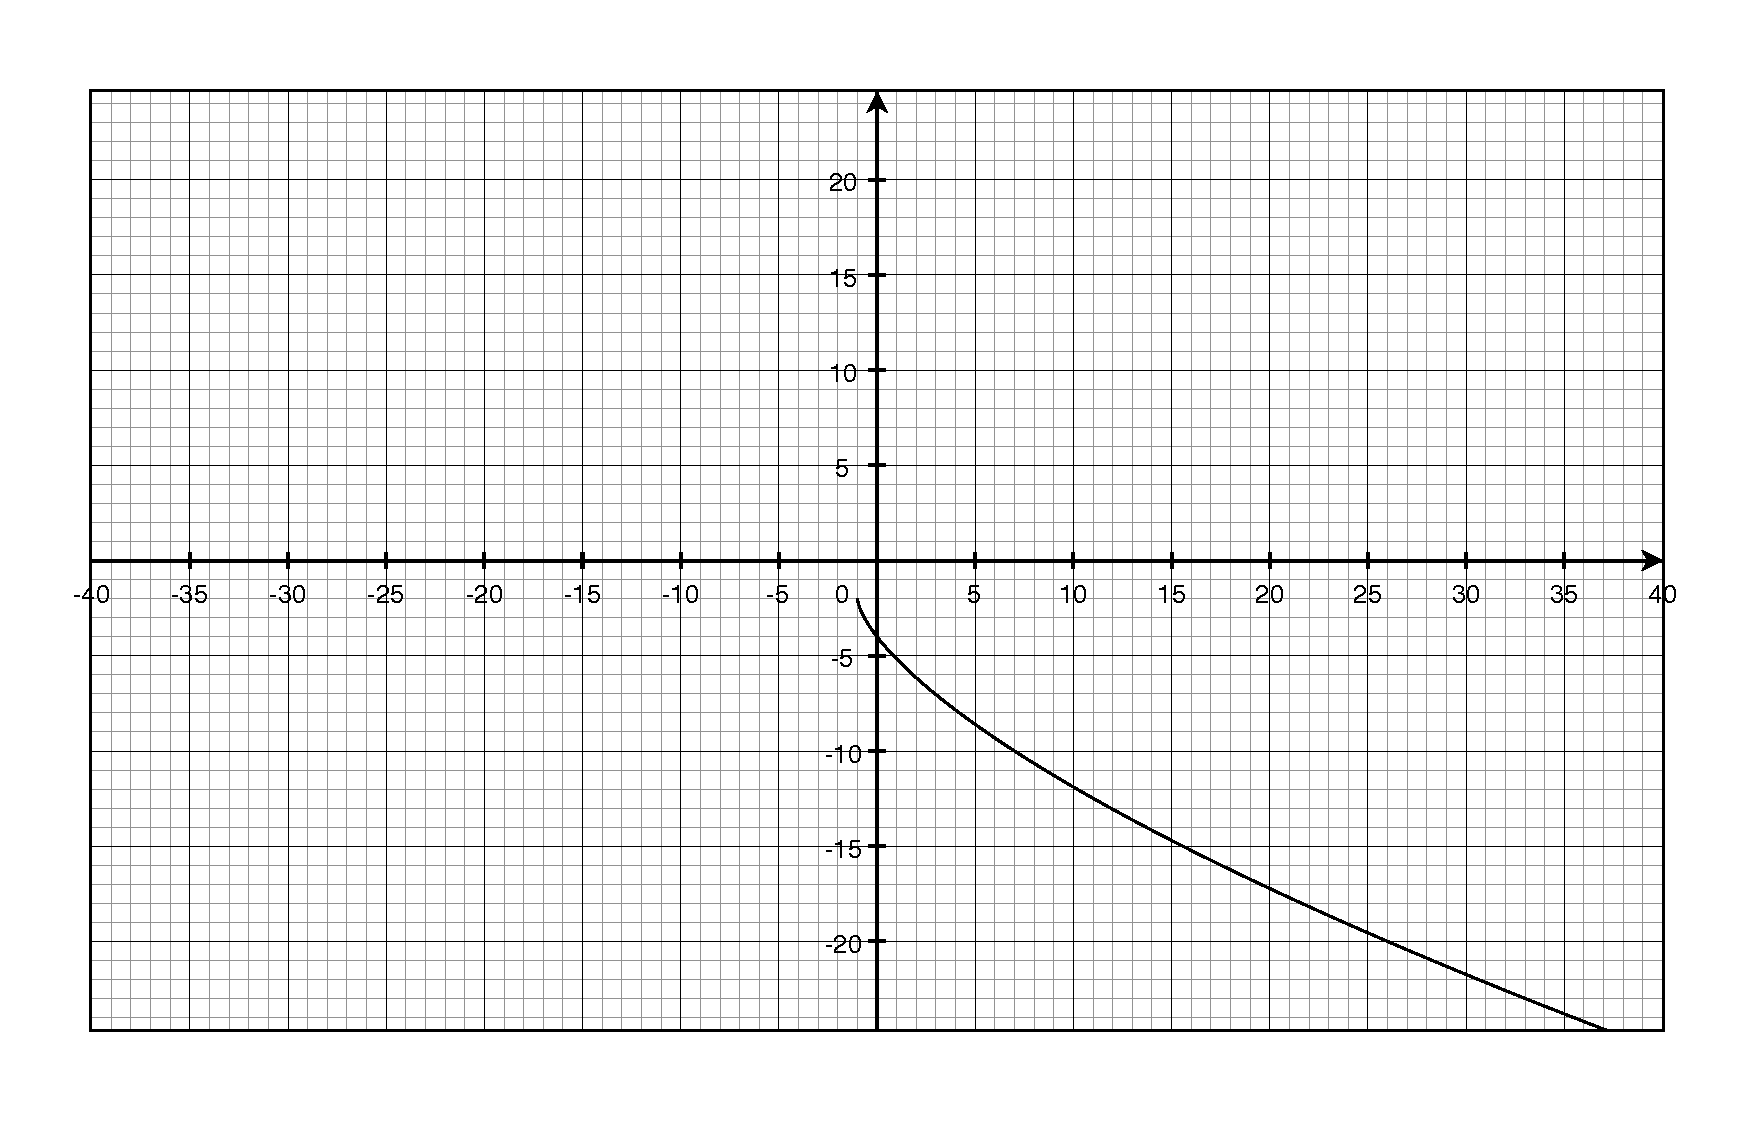
\includegraphics[scale=.3]{question9.eps}
  \caption*{Question 9}
\end{figure}

\item[10]
\begin{figure}[H]
  \centering
  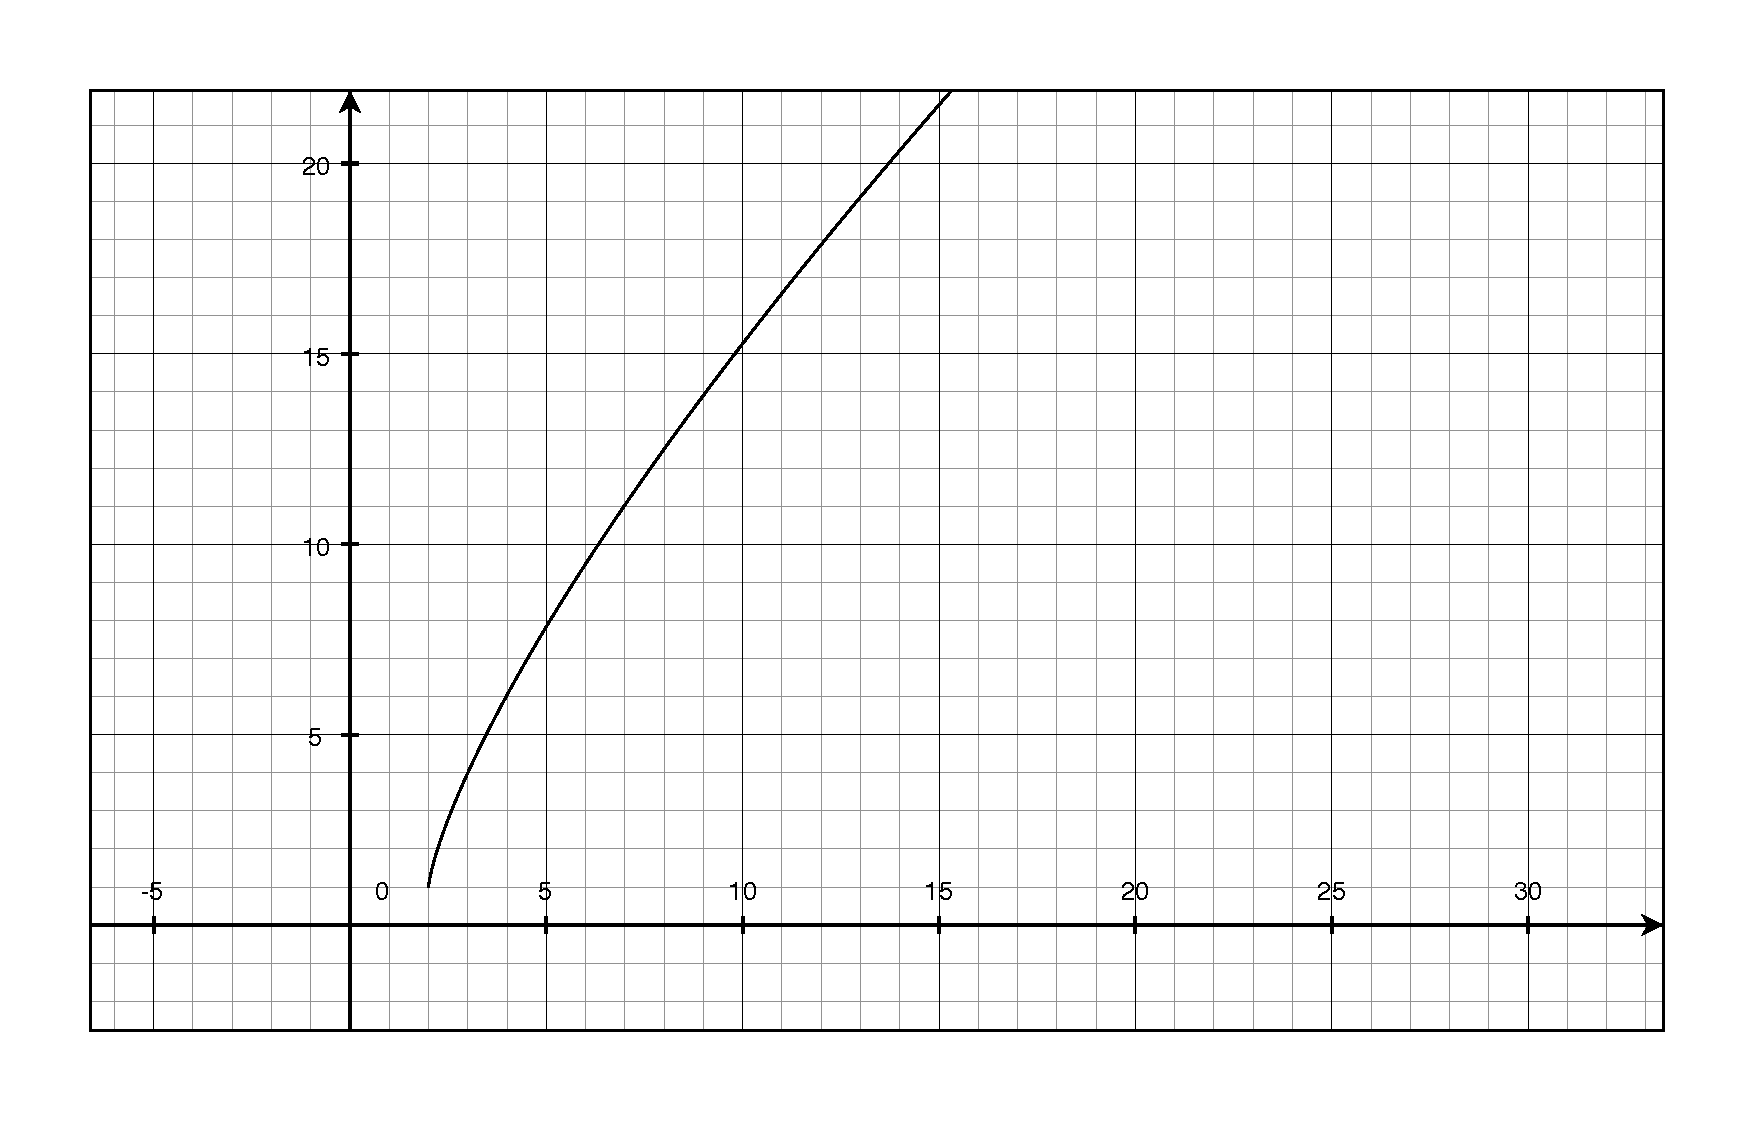
\includegraphics[scale=.3]{question10.eps}
  \caption*{Question 10}
\end{figure}

\item[13]
\begin{figure}[H]
  \centering
  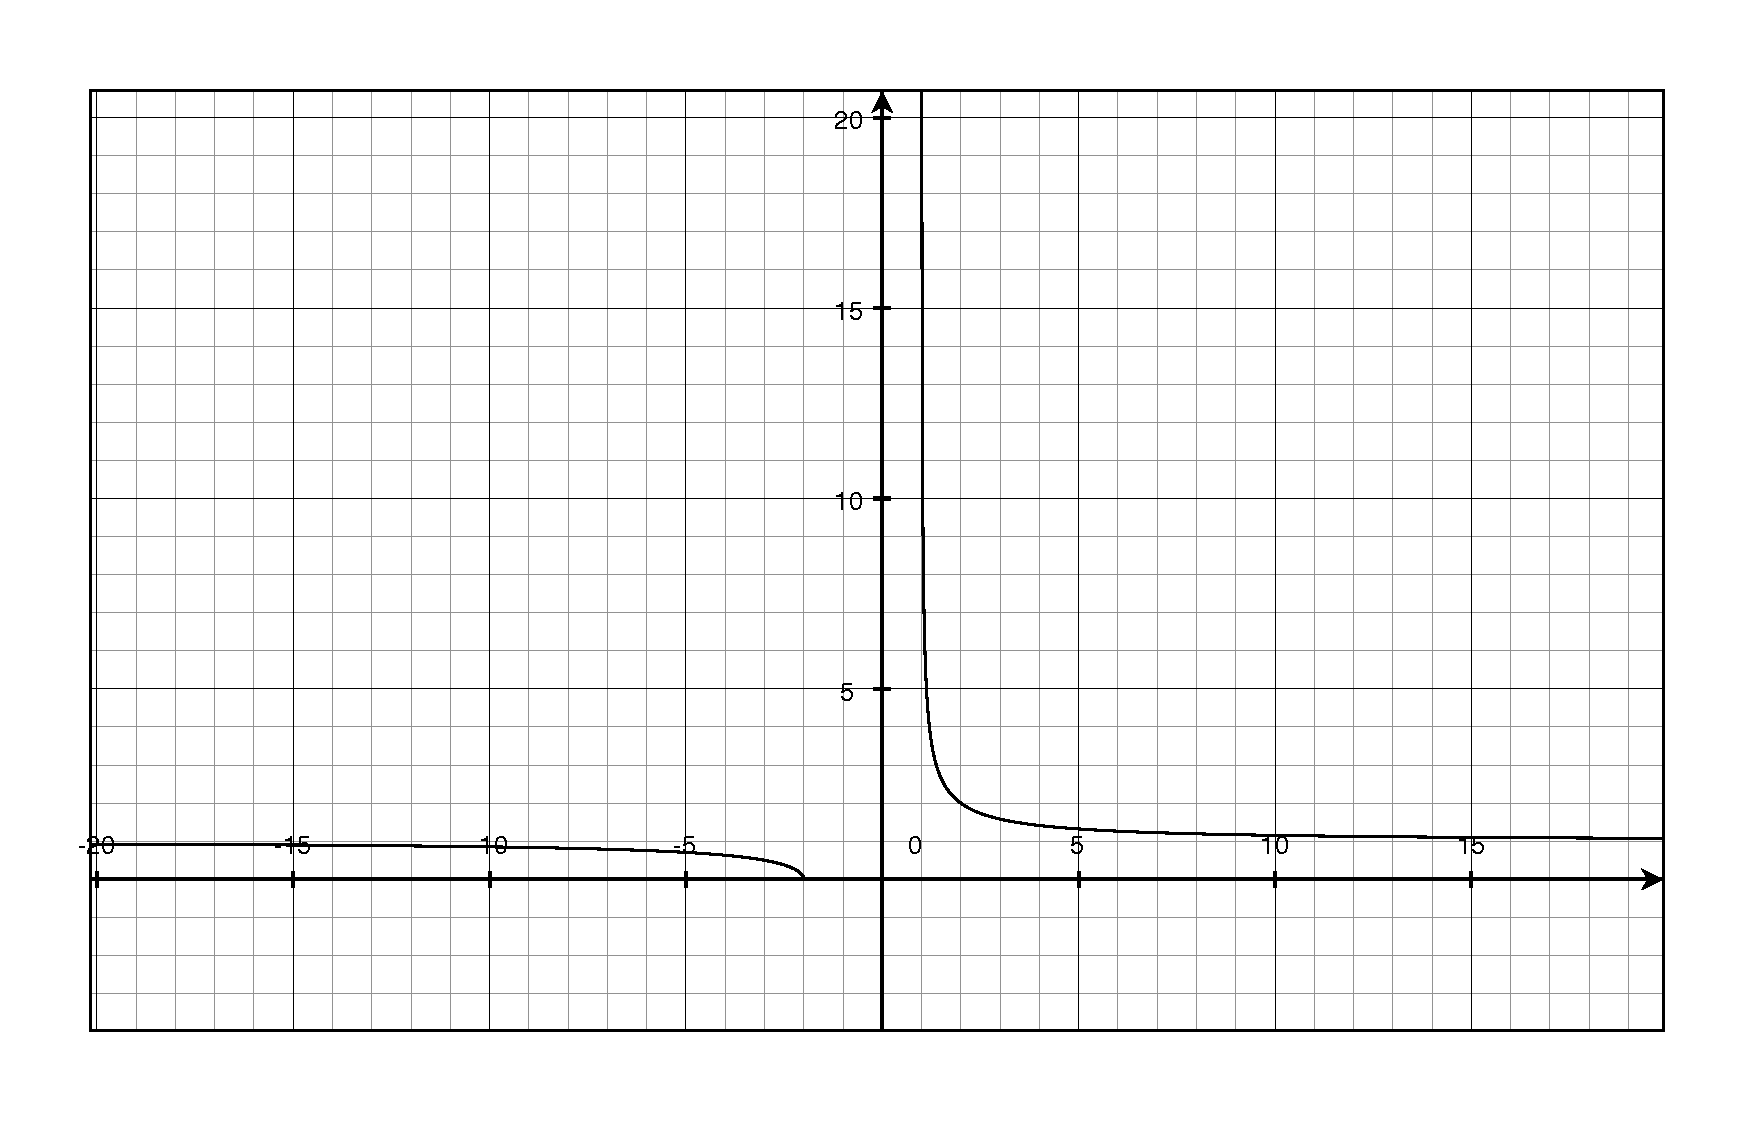
\includegraphics[scale=.3]{question13.eps}
  \caption*{Question 13}
\end{figure}

\end{description}

\ifprintanswers
\else

\vspace{4 in}

{\em I can't understand why people are frightened of new ideas. I'm frightened of the old ones.}

\vspace{.1 cm}
\hspace{1 cm} --John Cage
\fi
\end{document}

